\documentclass[12pt]{article}

\usepackage[portuguese]{babel}
\usepackage[utf8]{inputenc}
\usepackage{amsmath}
\usepackage{commath}
\usepackage[alf]{abntex2cite}
\usepackage{indentfirst}
\usepackage{graphicx}
\usepackage{multicol,lipsum}
\usepackage{subfig}
\usepackage{geometry}
\usepackage[alf]{abntex2cite}
\usepackage{subfig}

\geometry{
	paper = a4paper,
    inner = 3cm,
    outer = 3cm,
    top = 2cm,
    bottom = 2cm
}

\begin{document}
%\maketitle

\onehalfspacing

\begin{titlepage}
	\begin{center}

		\Huge{Universidade Federal de Alagoas}\\
		\large{Instituto de Computação}\\ 
		\large{Laboratório de Computação Científica e Análise Numérica}\\ 
        \vspace{220pt}
        \textbf{\LARGE{Relatório de acompanhamento de pesquisa}}\\
		%\title{{\large{Título}}}
		\vspace{3,5cm}
	\end{center}
	
	\begin{flushleft}
		\begin{tabbing}
			Aluno: Danilo Fernandes Costa\\
			Professor orientador: Alejandro Frery\\
	\end{tabbing}
 \end{flushleft}
	\vspace{1cm}
	
	\begin{center}
		\vspace{\fill}
			 Fevereiro\\
		 2019
			\end{center}
\end{titlepage}

\section{Introdução}

No presente relatório são apresentados alguns resultados obtidos da análise de regiões de solo com pouca ou nenhuma vegetação. Os dados PolSAR das regiões analisadas foram extraídas de uma imagem da Sierra del Lacandon National Park, Guatemala a qual foi adquirida em 10 de abril de 2015. Segue as imagens das regiões analisidas:

\begin{figure}[hbt]
    \centering
    \subfloat[Região 1]{{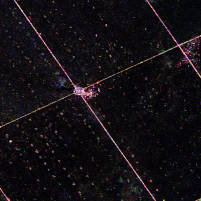
\includegraphics[width=0.4\linewidth]{../../Images/Report_19_02_27/ground_region1.png} }}%
    \qquad
    \subfloat[Região 2]{{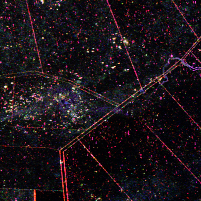
\includegraphics[width=0.4\linewidth]{../../Images/Report_19_02_27/ground_region2.png} }}%
    \vspace{0.05\linewidth}
    \subfloat[Região 3]{{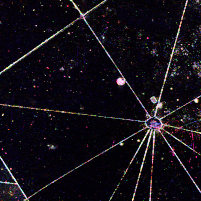
\includegraphics[width=0.4\linewidth]{../../Images/Report_19_02_27/ground_region3.png} }}%
    \qquad
    \subfloat[Região 4]{{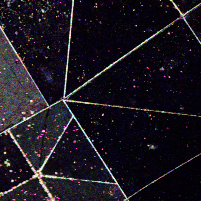
\includegraphics[width=0.4\linewidth]{../../Images/Report_19_02_27/ground_region4.png} }}%
    \caption{Regiões de solo analisadas}
    \label{fig:regions}
\end{figure}

\section{Análise das regiões de solo}

Inicialmente analisou-se nas regiões quais retroespalhadores apresentavam maior similaridade a seus dados. Para tal analisou-se o mapa de retroespalhadores elementares, o qual atribui a cada \textit{pixel} o retroespalhador elementar mais próximo em relação à distância geodésica, para cada uma das regiões -- os quais são apresentados na figuras \ref{fig:scatterer_map1} à \ref{fig:scatterer_map4} -- e constatou-se que \textit{random volume} é predominante.

\begin{figure}[!h]

  \centering
  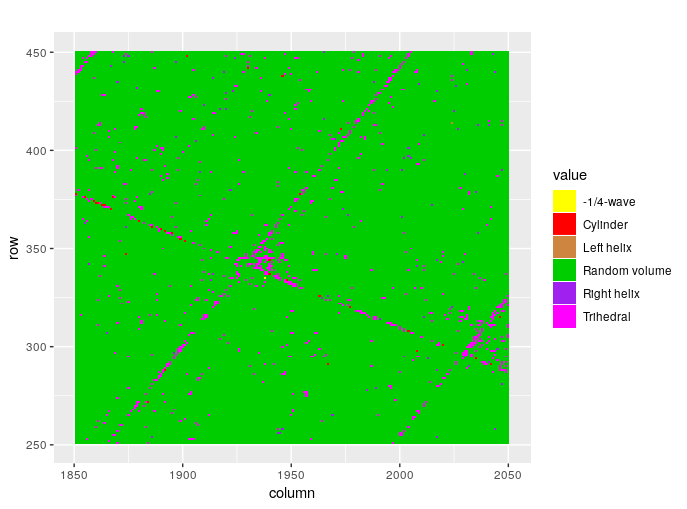
\includegraphics[width=\linewidth]{../../Images/Report_19_02_27/scatterer_map_region1.png}
  \caption{Mapa de retroespalhadores elementares da região 1}
  \label{fig:scatterer_map1}

\end{figure}

\begin{figure}[!h]

  \centering
  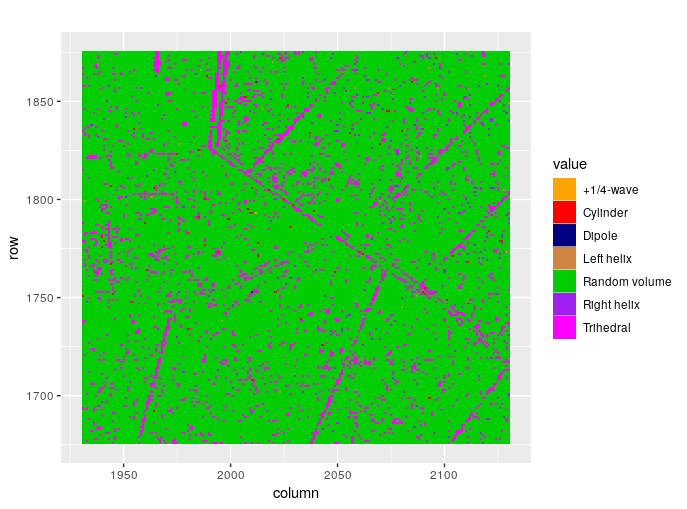
\includegraphics[width=\linewidth]{../../Images/Report_19_02_27/scatterer_map_region2.png}
  \caption{Mapa de retroespalhadores elementares da região 2}
  \label{fig:scatterer_map2}

\end{figure}

\newpage

\begin{figure}[!h]

  \centering
  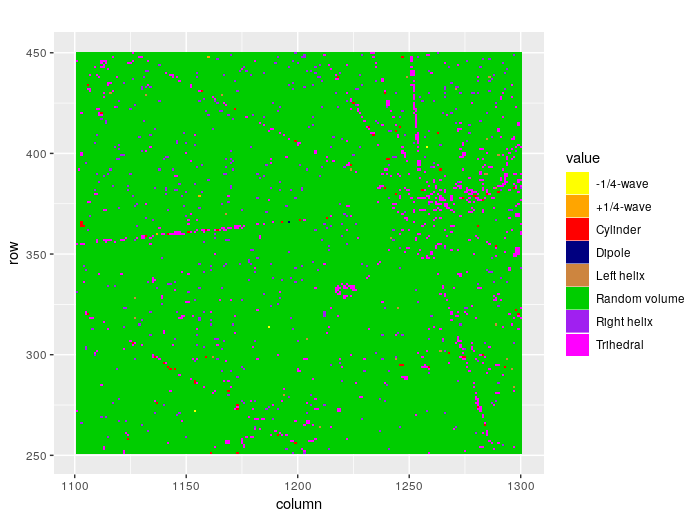
\includegraphics[width=\linewidth]{../../Images/Report_19_02_27/scatterer_map_region3.png}
  \caption{Mapa de retroespalhadores elementares da região 3}
  \label{fig:scatterer_map3}

\end{figure}

\begin{figure}[!h]

  \centering
  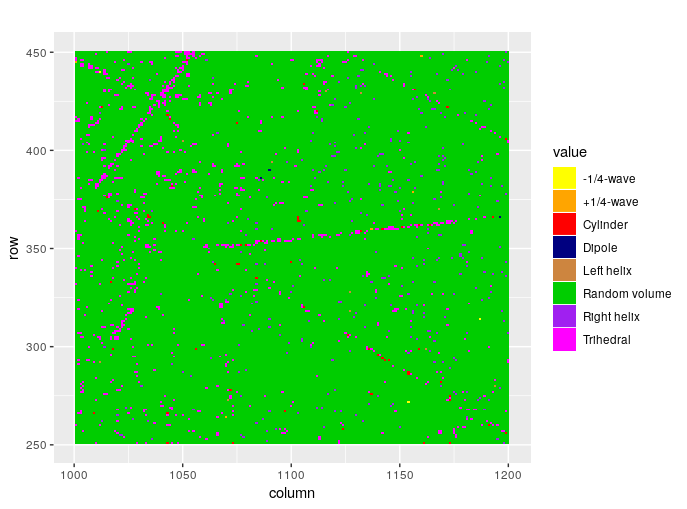
\includegraphics[width=\linewidth]{../../Images/Report_19_02_27/scatterer_map_region4.png}
  \caption{Mapa de retroespalhadores elementares da região 4}
  \label{fig:scatterer_map4}

\end{figure}

\newpage

Ao analisar-se os histogramas das similaridades em relação a \textit{random volume} das regiões 1 e 2, os quais apresentam-se nas figuras \ref{fig:hist_beta_rv1} e \ref{fig:hist_beta_rv2}, observou-se a semelhança entre os histogramas e o ajuste a distribuição beta. 

\begin{figure}[!h]

  \centering
  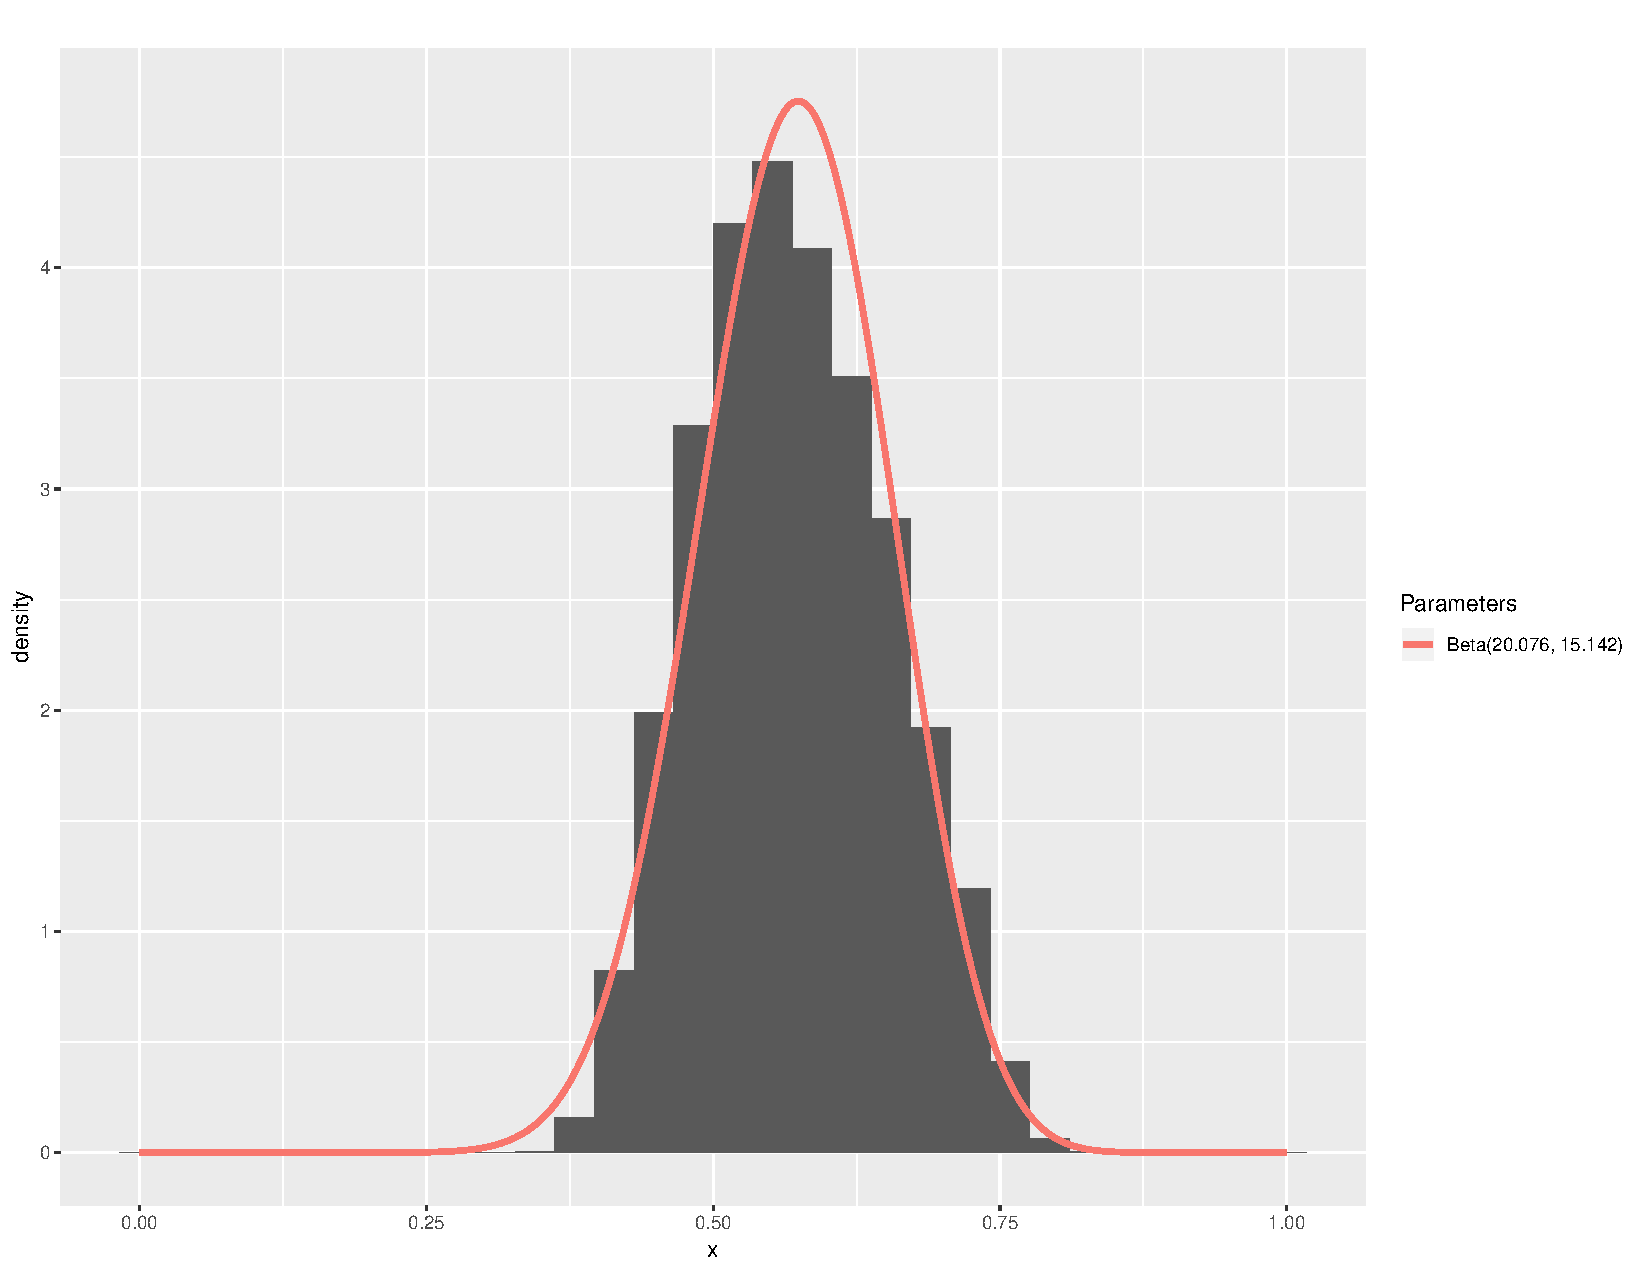
\includegraphics[width=0.8\linewidth]{../../Figures/Report_19_02_27/hist_rv_beta_region1.pdf}
  \caption{Histograma das similaridades dos dados da região 1 a \textit{random volume}}
  \label{fig:hist_beta_rv1}

\end{figure}

\begin{figure}[!h]

  \centering
  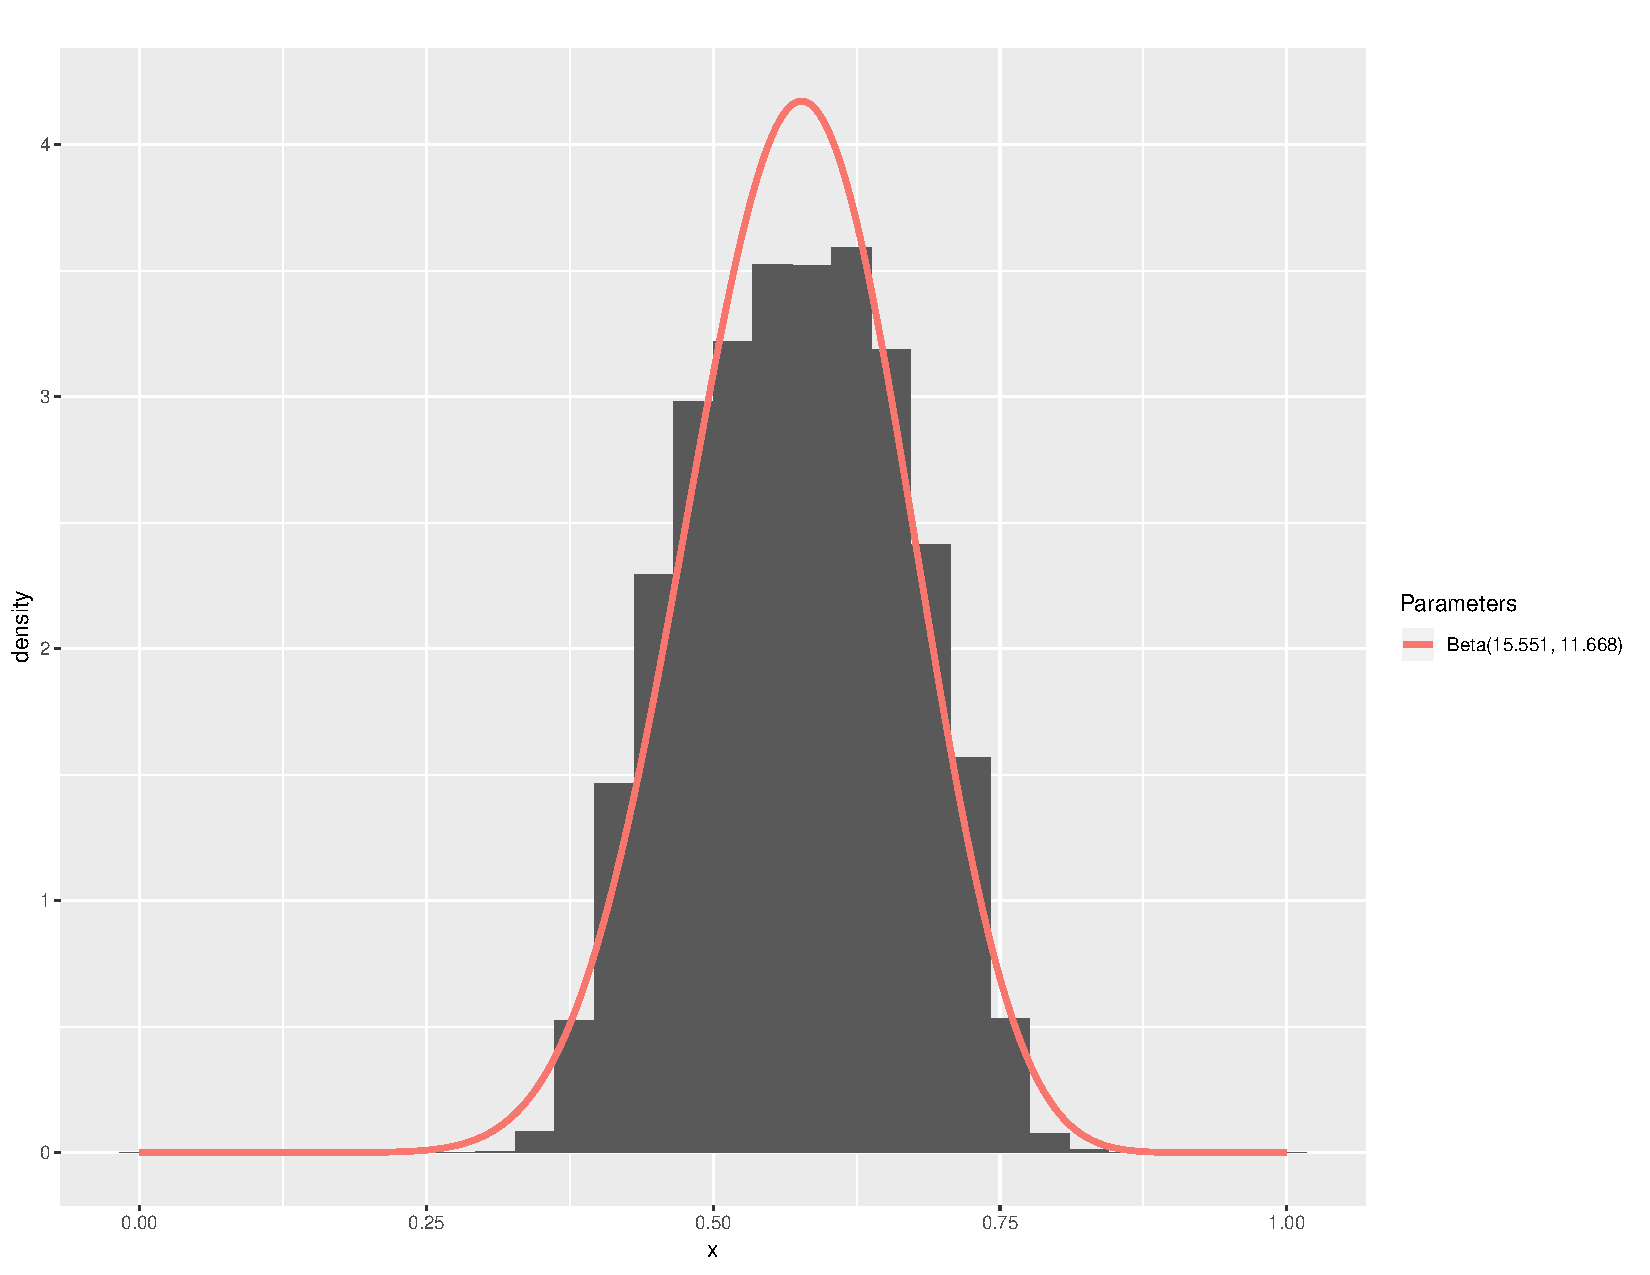
\includegraphics[width=0.8\linewidth]{../../Figures/Report_19_02_27/hist_rv_beta_region2.pdf}
  \caption{Histograma das similaridades dos dados da região 2 a \textit{random volume}}
  \label{fig:hist_beta_rv2}

\end{figure}

Embora haja considerável distância entre os parâmetros estimados da distribuição beta nas figuras \ref{fig:hist_beta_rv1} e \ref{fig:hist_beta_rv2}, as médias, os desvios padrões e o formato dos histogramas são similares. Isto pode ser observado nas figuras \ref{fig:hist_norm_rv1} e \ref{fig:hist_norm_rv2}. Dessa forma, constatou-se que os parâmetros da distribuição beta são muito sensíveis a variações na média e desvio padrão.

\begin{figure}[!h]

  \centering
  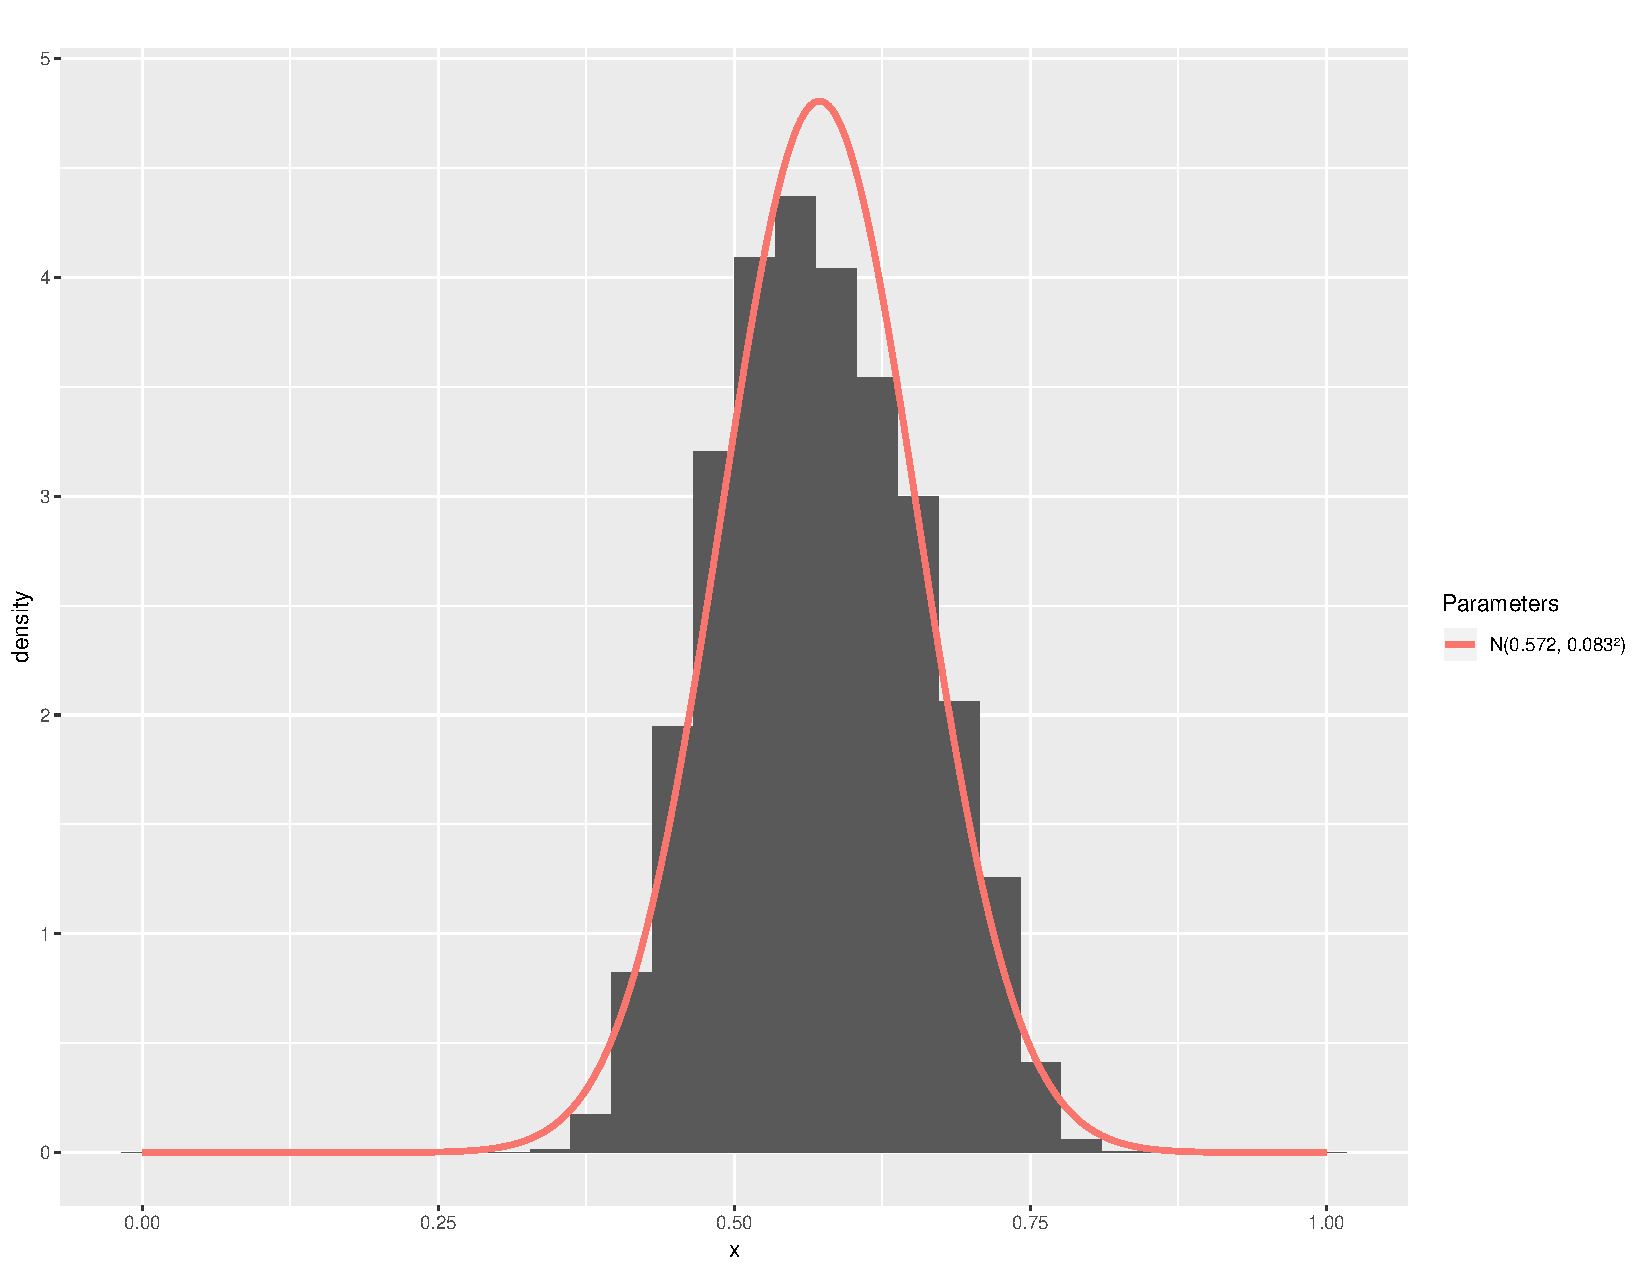
\includegraphics[width=0.8\linewidth]{../../Figures/Report_19_02_27/hist_rv_norm_region1.pdf}
  \caption{Histograma das similaridades dos dados da região 1 a \textit{random volume}}
  \label{fig:hist_norm_rv1}

\end{figure}

\begin{figure}[!h]

  \centering
  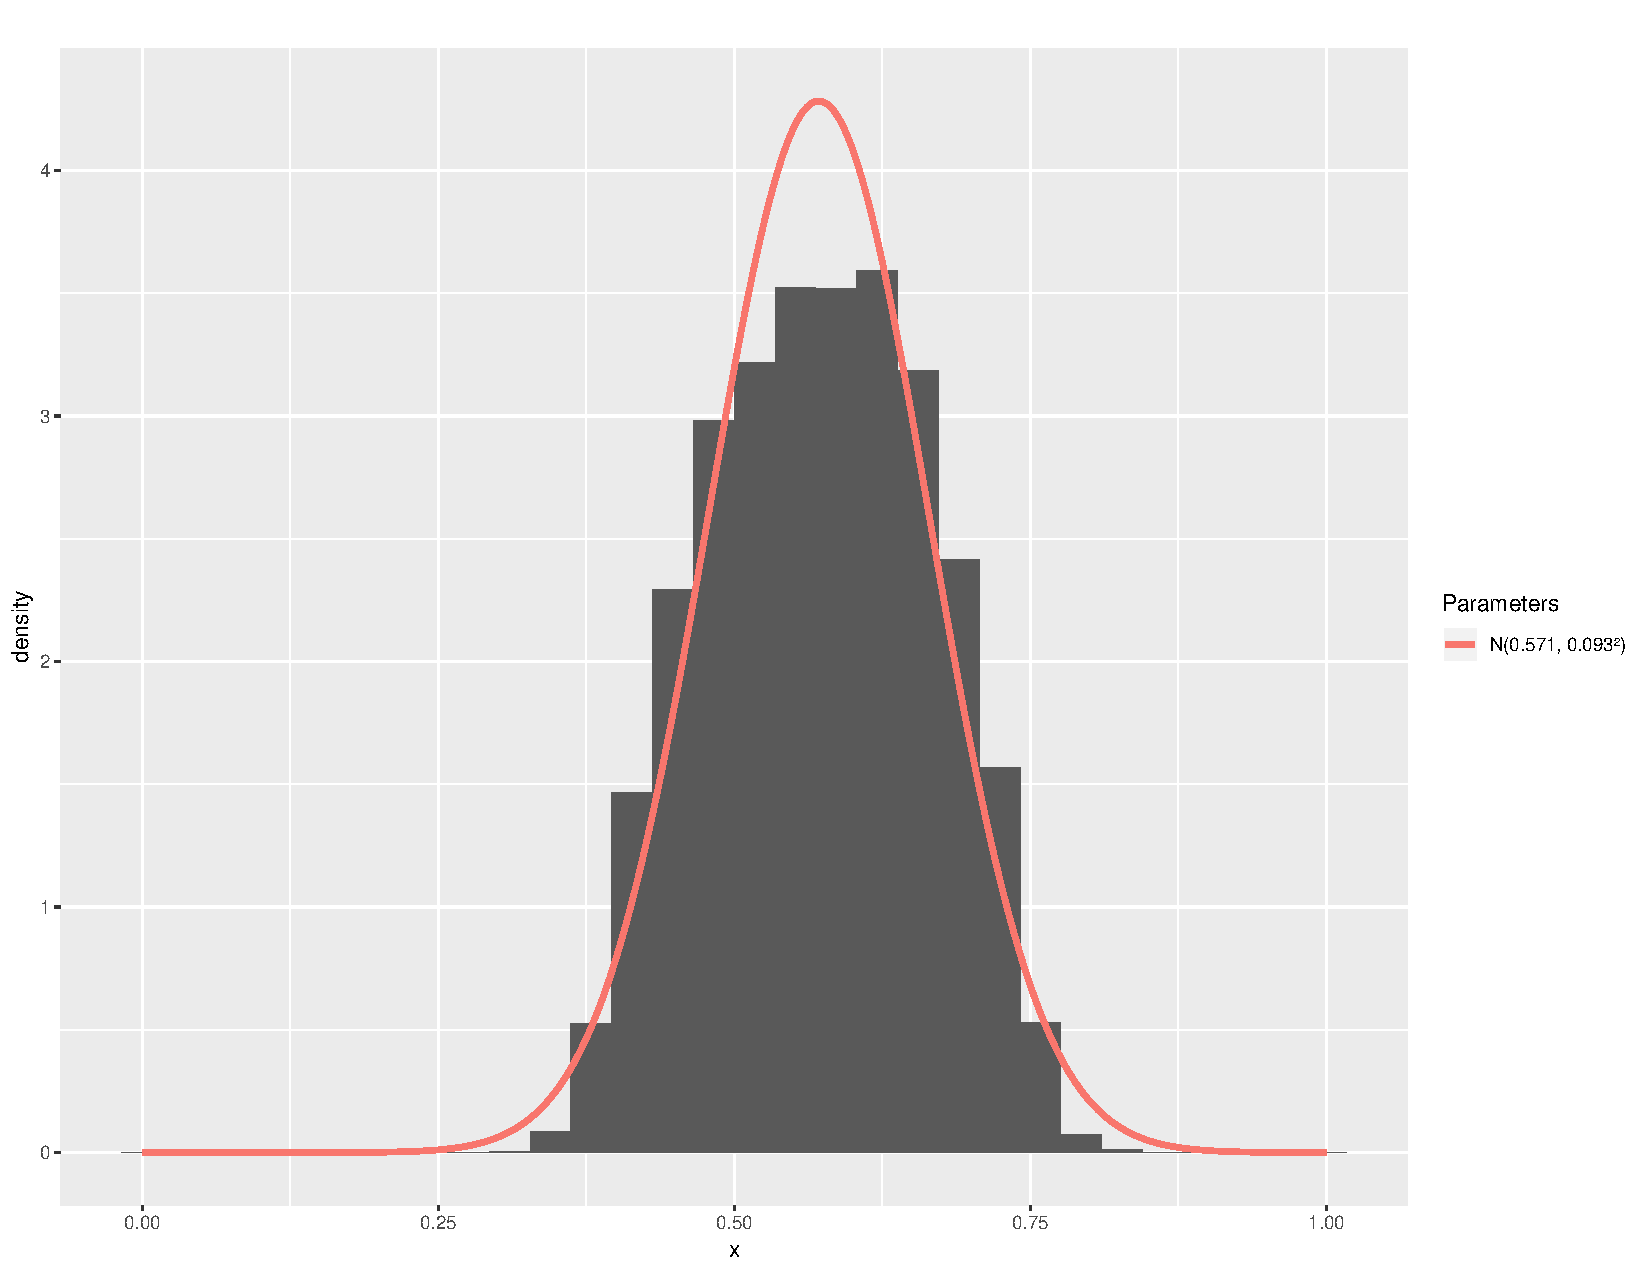
\includegraphics[width=0.8\linewidth]{../../Figures/Report_19_02_27/hist_rv_norm_region2.pdf}
  \caption{Histograma das similaridades dos dados da região 2 a \textit{random volume}}
  \label{fig:hist_norm_rv2}

\end{figure}

Comparando esses resultados com aqueles obtidos para regiões de vegetação e observando as imagens das regiões, pôde-se supor que essas regiões apresentam um pequeno grau vegetação.

Ao obter-se os \textit{heatmaps} das similaridades em relação a \textit{random volume} das quatro regiões observou-se que as regiões 1 e 2 apresentavam homogeneidade nos mesmos, diferentemente das outras duas, como pode ser observado nas imagens \ref{fig:heat_rv1} a \ref{fig:heat_rv4}. A justificativa é a existência de regiões com diferentes comportamentos de espalhamento, ou seja, diferentes níveis de vegetação.

\begin{figure}[!h]

  \centering
  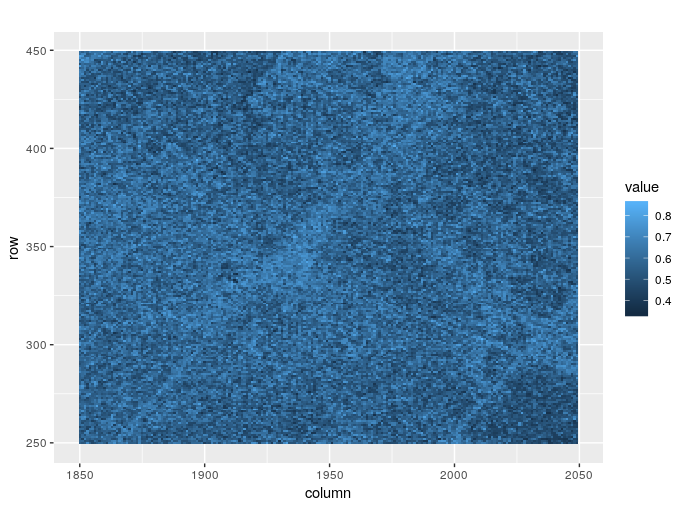
\includegraphics[width=0.8\linewidth]{../../Images/Report_19_02_27/heatmap_rv_region1.png}
  \caption{\textit{heatmap} das similaridades da região 1 em relação a \textit{random volume}}
  \label{fig:heat_rv1}

\end{figure}

\begin{figure}[!h]

  \centering
  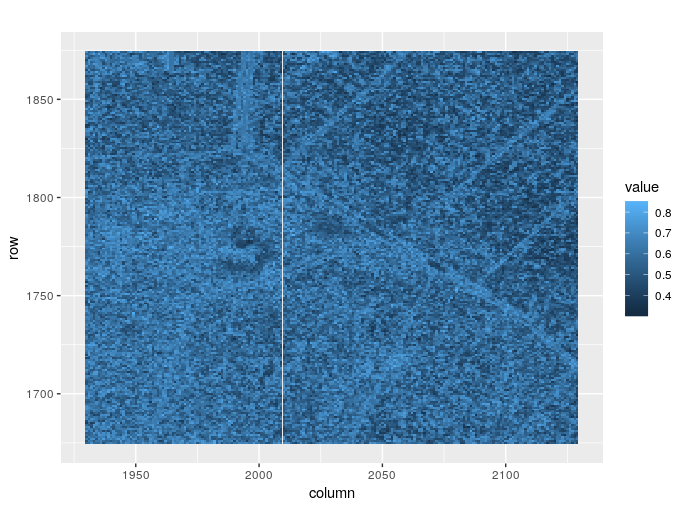
\includegraphics[width=0.8\linewidth]{../../Images/Report_19_02_27/heatmap_rv_region2.png}
  \caption{\textit{heatmap} das similaridades da região 2 em relação a \textit{random volume}}
  \label{fig:heat_rv2}

\end{figure}

\newpage

\begin{figure}[!h]

  \centering
  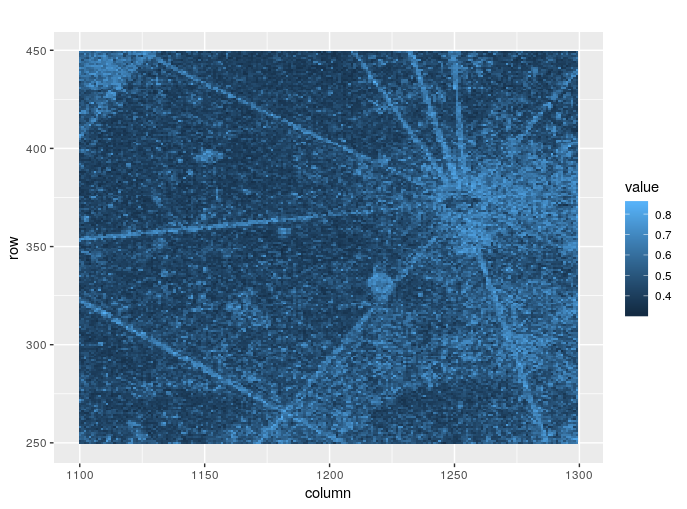
\includegraphics[width=0.8\linewidth]{../../Images/Report_19_02_27/heatmap_rv_region3.png}
  \caption{\textit{heatmap} das similaridades da região 3 em relação a \textit{random volume}}
  \label{fig:heat_rv3}

\end{figure}

\begin{figure}[!h]

  \centering
  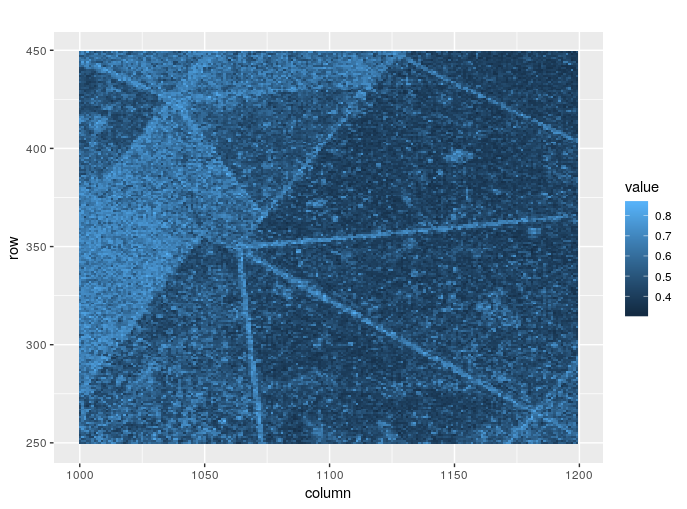
\includegraphics[width=0.8\linewidth]{../../Images/Report_19_02_27/heatmap_rv_region4.png}
  \caption{\textit{heatmap} das similaridades da região 4 em relação a \textit{random volume}}
  \label{fig:heat_rv4}

\end{figure}

\newpage

Nestas duas últimas, ao comparar com as imagens das regiões, observou-se que as subregiões homogêneas e mais escuras no \textit{heatmap} correspondem possivelmente a regiões de solo exposto. Ao analisar uma subregião em cada uma das regiões 3 e 4 com essas características obteve-se os seguintes histogramas, os quais são similares e ajustam-se à função de densidade da distribuição PERT com parâmetros similares.

\begin{figure}[!h]

  \centering
  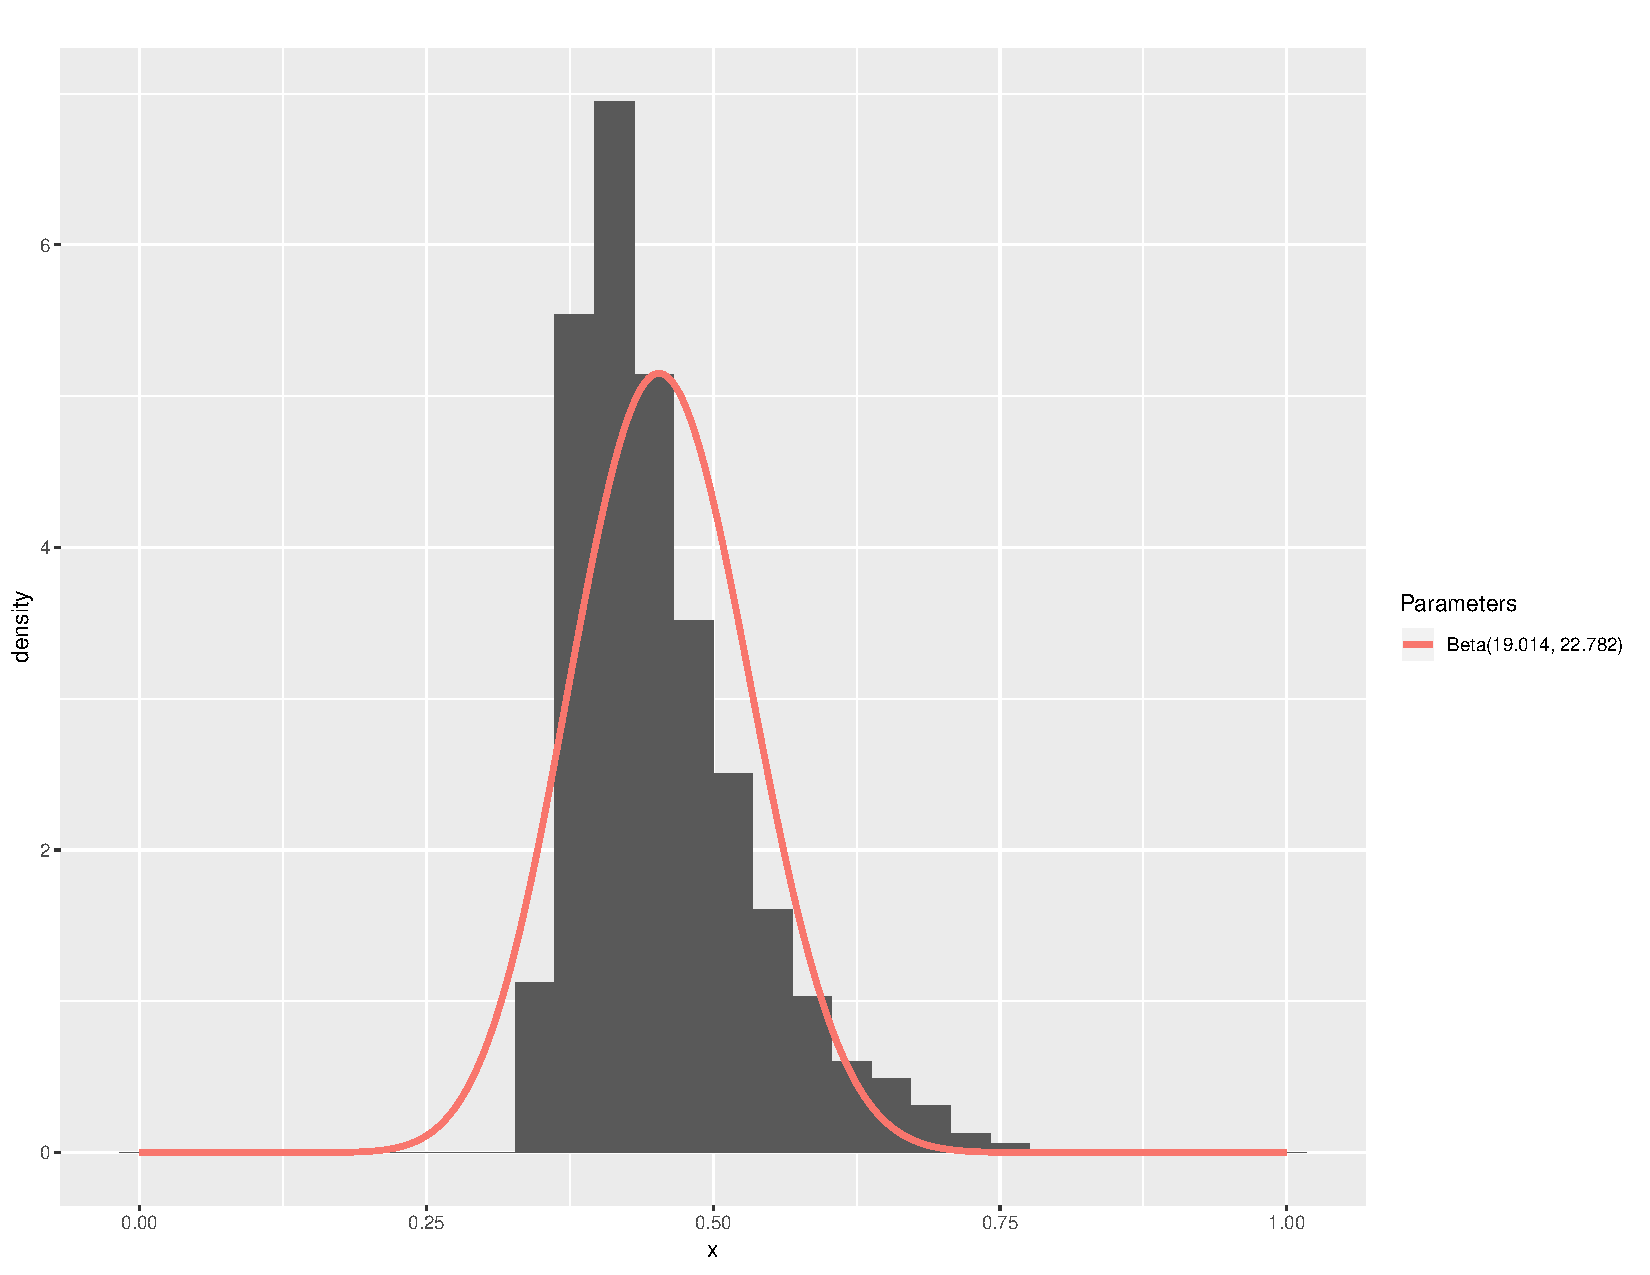
\includegraphics[width=0.75\linewidth]{../../Figures/Report_19_02_27/hist_rv_subregion3.pdf}
  \caption{Histograma das similaridades dos dados de uma subregião de solo exposto da região 3 a \textit{random volume}}
  \label{fig:hist_sub_rv3}

\end{figure}

\begin{figure}[!h]

  \centering
  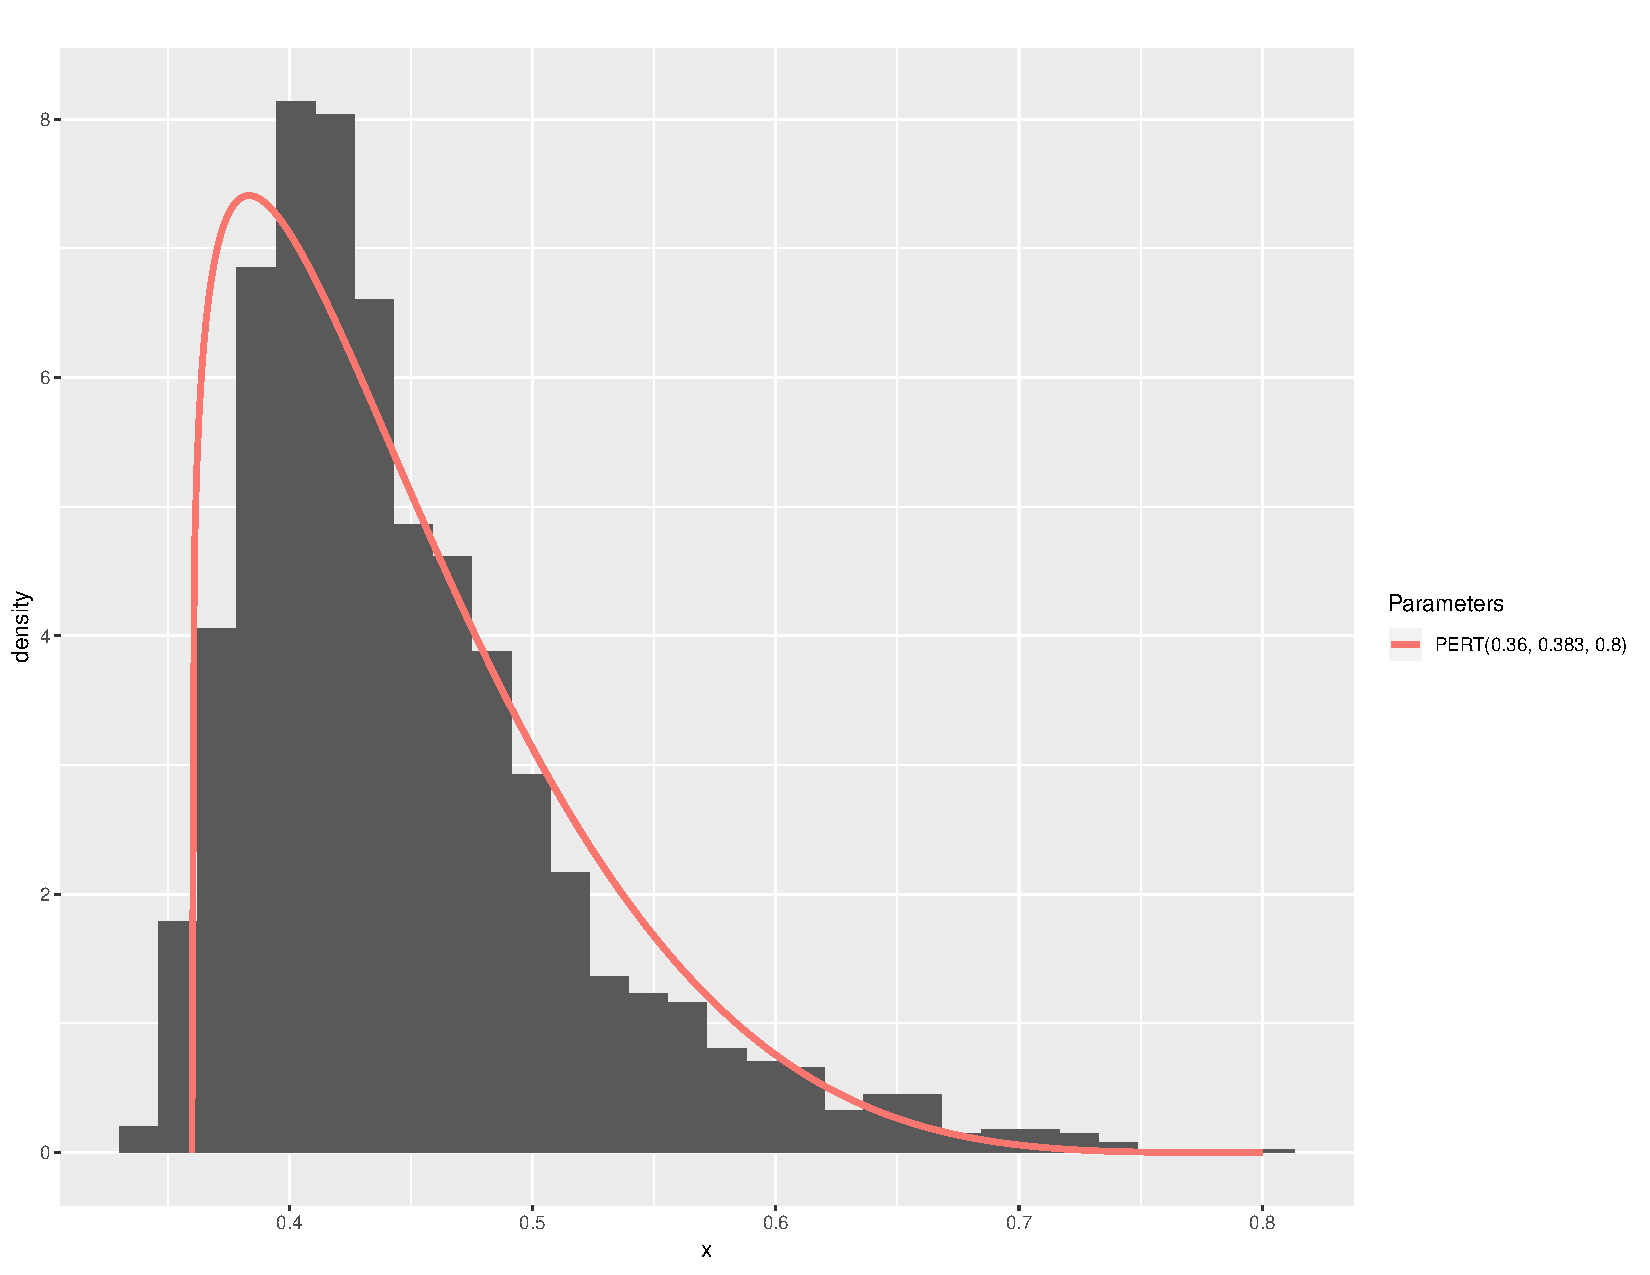
\includegraphics[width=0.75\linewidth]{../../Figures/Report_19_02_27/hist_rv_subregion4.pdf}
  \caption{Histograma das similaridades dos dados de uma subregião de solo exposto da região 4 a \textit{random volume}}
  \label{fig:hist_sub_rv4.1}

\end{figure}

Ao analisar uma subregião da região 4 que apresenta-se mais clara no \textit{heatmap}, obteve-se o histograma da figura \ref{fig:hist_sub_rv4.2} o qual ajusta a distribuição beta e assemalha-se aos histogramas das regiões 1 e 2. Por isso, supõe-se que essa subregião apresente alguma vegetação.

\begin{figure}[!h]

  \centering
  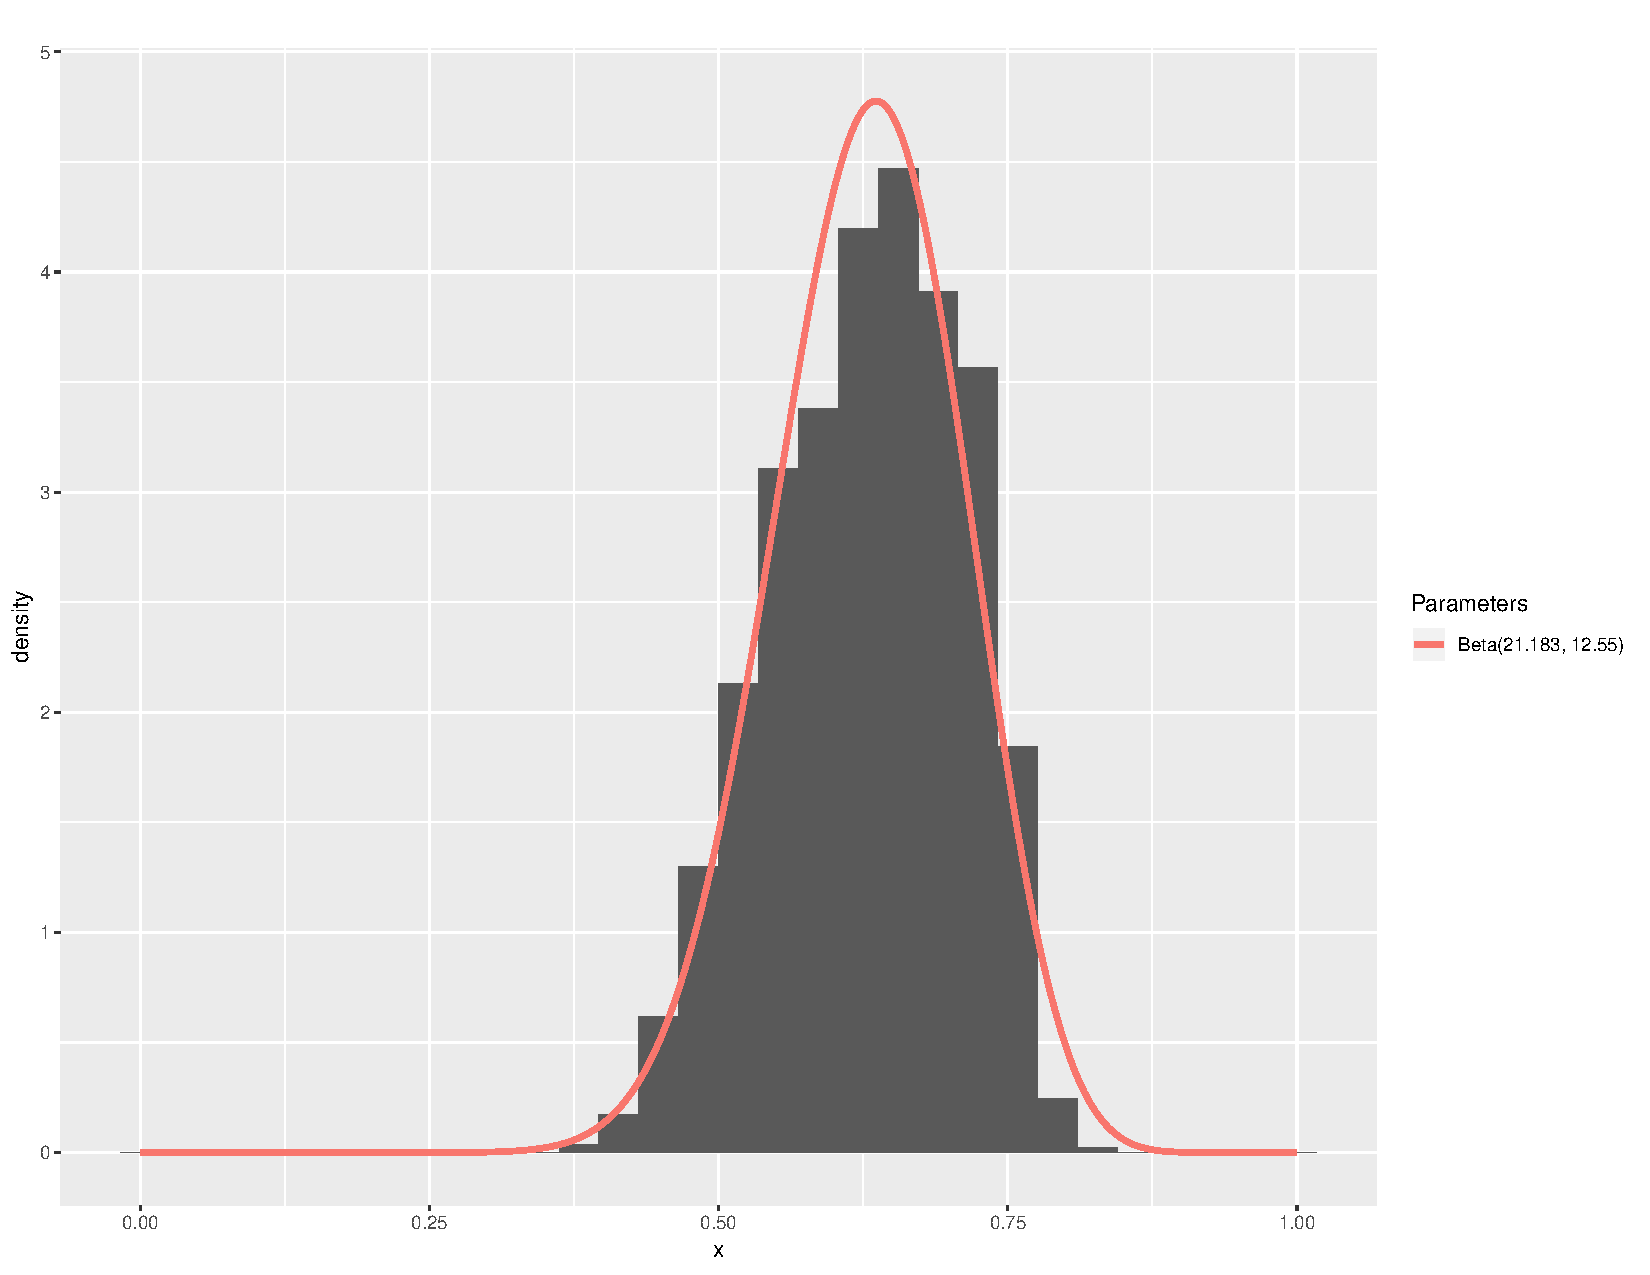
\includegraphics[width=0.75\linewidth]{../../Figures/Report_19_02_27/hist_rv_subregion4_2.pdf}
  \caption{Histograma das similaridades dos dados de uma subregião da região 4 a \textit{random volume}}
  \label{fig:hist_sub_rv4.2}

\end{figure}


\section{Conclusão}

Analisando os resultados dispostos no presente relatório, concluí-se que a similaridade dos dados de regiões de solo exposto em relação ao retroespalhador prototípico \textit{random volume} apresenta um comportamento estatístico que pode ser modelado por uma distribuição de probabilidade e que difere do comportamento observado em regiões com alguma vegetação. Portanto, é possível distinguir regiões de solo exposto de regiões com vegetação por meio da Distância Geodésica de seus dados a \textit{random volume}.

Os próximos passos consistirão em
\begin{itemize}
  \item observar o comportamento da similaridade entre os dados de regiões de solo exposto e outros retroespalhadores.
\end{itemize}
\end{document}